\section{Hash cracking}

\subsection{Hash 1 (20p)}
\addtocounter{points}{20}
I do believe I'll be a tail fin hero on Norwegian in 50 years :) I travelled on a plane a few years ago, when I had to create my password, so I used the name on the tail. Here's the hash: 4b57b34a1855d0d9137d36023156717c What was my password?

\textbf{Solution:}\\
I first gathered a \href{https://en.wikipedia.org/wiki/List_of_Norwegian_Air_Shuttle_tail_fin_heroes_and_fleet}{list of the names of the people who are on the tail fin of Norwegian's planes}.

\begin{center}
    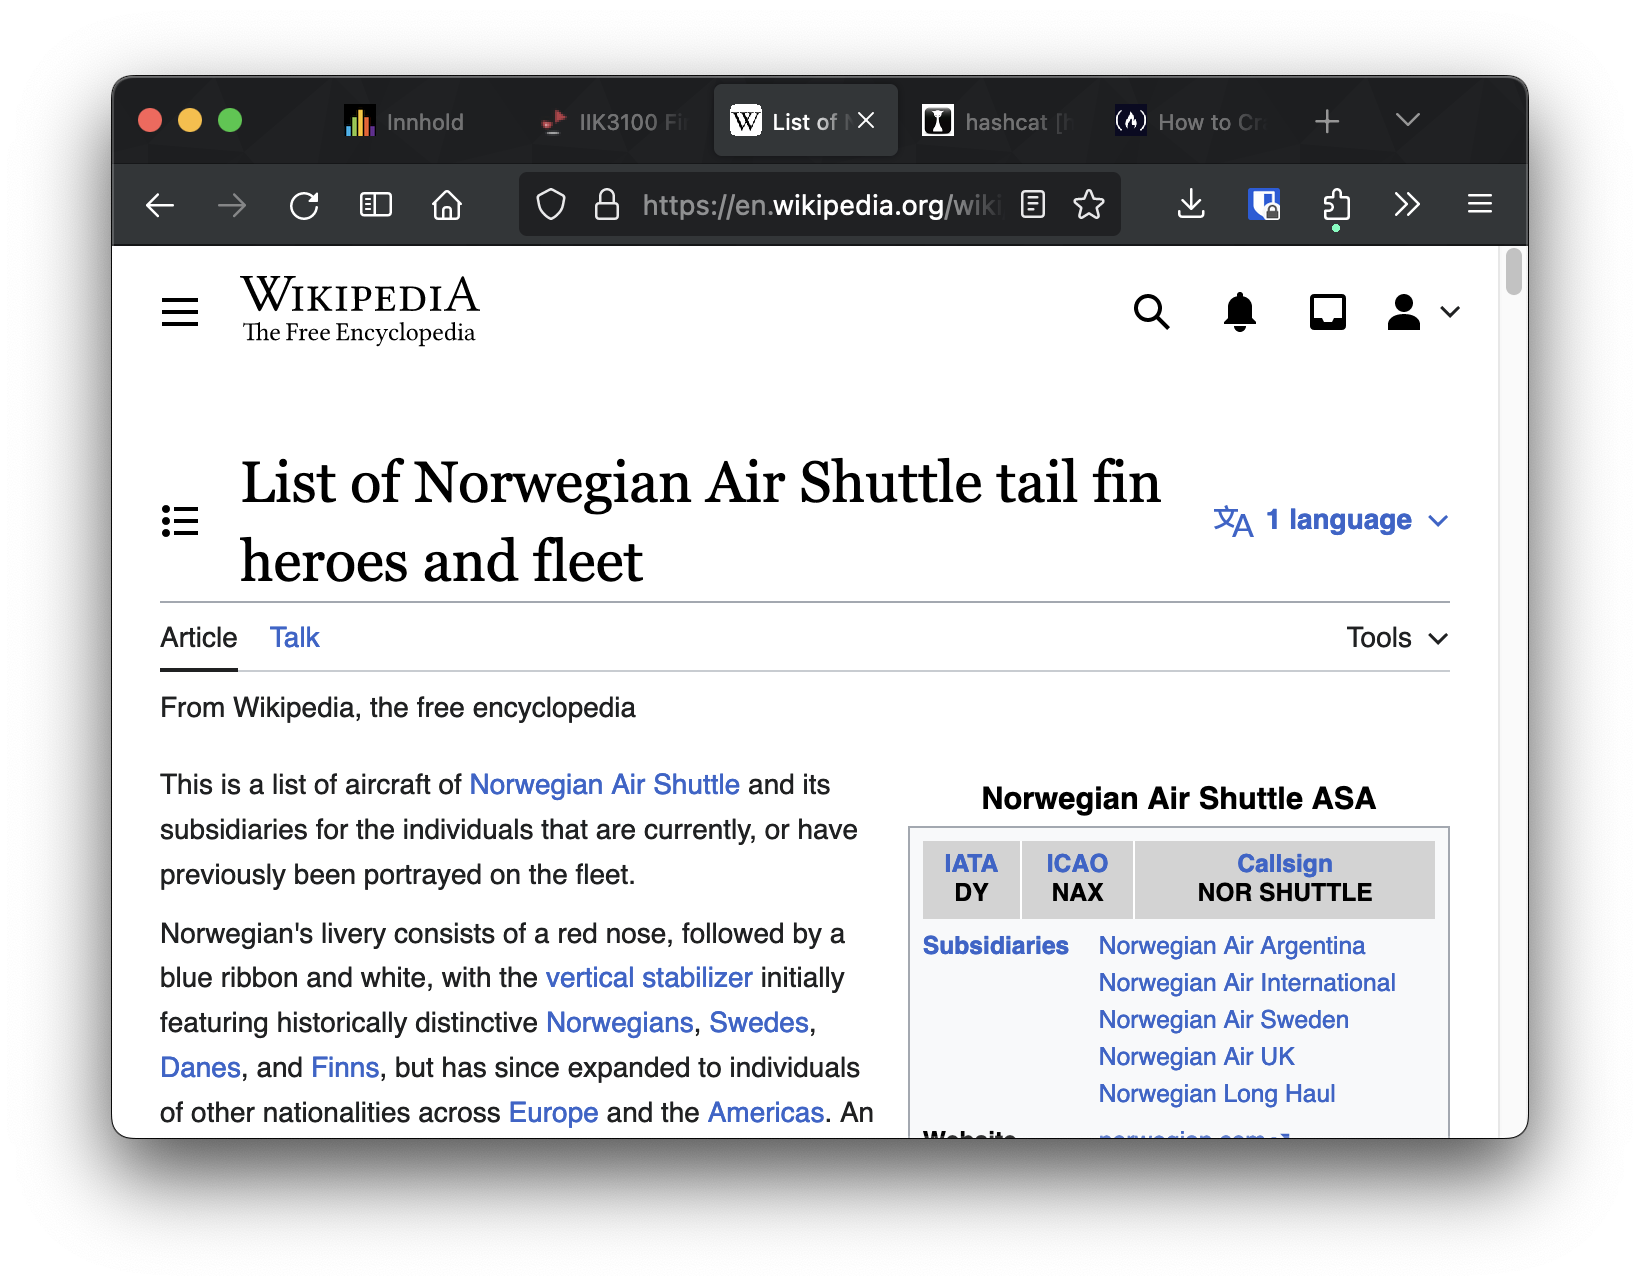
\includegraphics[width=10cm]{img/Hash cracking/Hash1/Screenshot 2023-11-24 at 10.47.35.png}
\end{center}

Then using hashcat I cracked the hash using the wordlist I created from the list of names.

\begin{center}
    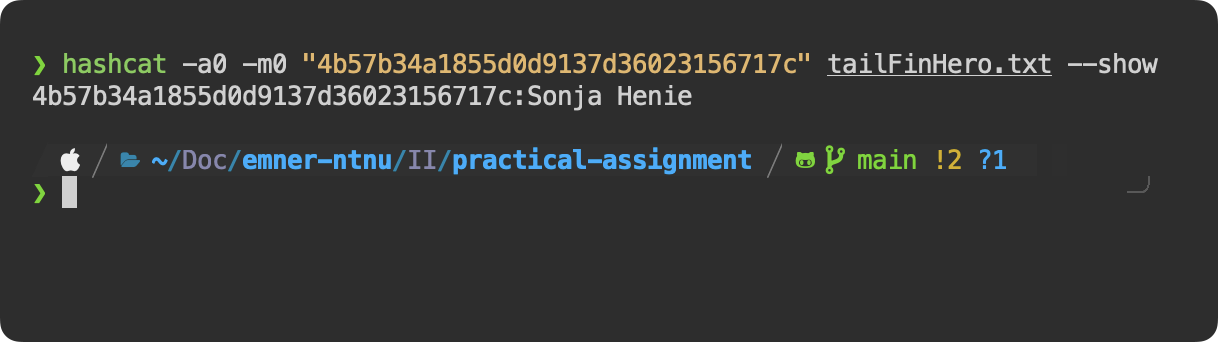
\includegraphics[width=15cm]{img/Hash cracking/Hash1/Screenshot 2023-11-24 at 10.46.31.png}
\end{center}

The password was \texttt{Sonja Henie}.

\newpage
\subsection{Hash 2 (20p)}
\addtocounter{points}{20}
My last idea of inventing a brilliant hashing did not work. Many of you could crack it. But I don't give up, here's the new idea: I convert my password to hexa then I hash it, e.g:

Julie \(\rightarrow\) 4A756C6965 \(\rightarrow\) 19225f5d4e8beefd1bb5374a4a1b92f1

Here's my hash: 49c6a1526a77b34a64e2feaa7dffccd1

\textbf{Solution:}\\
I solved this task using a python script. First I imported the \texttt{rockyou} wordlist.
Then I created a function that hashes a password using the same method as the hash in the task.
Then I created a function that iterates over the passwords in the wordlist and compares the hashes, and if they match it returns the password.

\begin{minted}
[
frame=lines,
framesep=2mm,
baselinestretch=1.2,
fontsize=\footnotesize,
linenos
]
{python}
import hashlib
from itertools import product
from string import ascii_lowercase, ascii_uppercase

to_be_cracked = "49c6a1526a77b34a64e2feaa7dffccd1"
passwd_list = open("rockyou.txt", "r", encoding="latin-1").readlines()

def hash(password: str) -> str:
    passwd = password.encode('utf-8')  # encode to utf-8
    hexa = passwd.hex().upper()  # convert to hexadecimal and uppercase
    hashed = hashlib.md5(hexa.encode('utf-8')).hexdigest() # hash the hexadecimal
    return hashed

def crack(h: str) -> str:
    for passwd in passwd_list: # iterate over the passwords
        passwd = passwd.strip() # remove whitespaces
        if hash(passwd) == h: # compare the hashes
            return passwd # return the password

print(crack(to_be_cracked)) # print the cracked password
\end{minted}

The password was \texttt{Shine}.

\newpage
\subsection{Hash 3 (30p)}
\addtocounter{points}{30}
I managed to dump the users table :)

id, user, pwd, salt 1, admin, 610a2ee688cda9e724885e23cd2cfdee, key 33, sam, 56a03849f5d1b03353f22f64f04bd143, Julie

Can you tell me what is Sam's password. I know him a bit, he's crazy about Take that and the song Julie. How lucky he is, his salt is also Julie.

\textbf{Solution:}\\
To solve this tash I used hashcat with the hash mode for md5(\$pass.\$salt) and the rockyou wordlist.
Running the command 
\\\texttt{hashcat -a0 -m10 "56a03849f5d1b03353f22f64f04bd143:Julie" rockyou.txt} resulted in the following output:

\begin{center}
    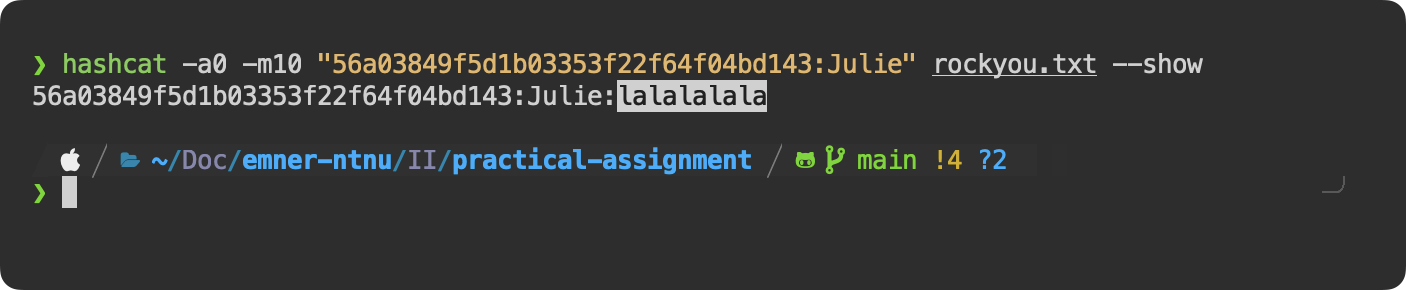
\includegraphics[width=15cm]{img/Hash cracking/Hash3/Screenshot 2023-11-24 at 23.05.42.png}
\end{center}

The password was \texttt{lalalalala}.
